\documentclass{article}
\usepackage[section]{placeins}
\usepackage{graphicx}

\author{Yaghoub Shahmari}
\title{Report - Problem Set no 2}
\date{\today}
\graphicspath{ {../Figs/} }

\begin{document}
    \maketitle
    \section*{Problem 1}
    \textbf{Basic description:}

    We introduce the $F_{(a)}=a^{2}+C$ as our basic form of complex transmission.
    In order to fulfill our desire,
    we have to create our coordinate plane using two loops and in each loop,
    we will cover an axis (our axes are actually a one-dimensional array that
    contains a range of numbers). Then we have to choose a single point on our
    complex coordinates plane and transmit it using a loop, n times and save
    the norm value of our final number. Then we have to check if the value is
    smaller than K (which is equal to $\frac{1+\sqrt{1+4 \cdot c}}{2}$). If it was, then we must keep the
    value equal to K. So we will have an array that contains real values.
    And finally,
    we will use the functions that draw us a heatmap of a 2D array.
    Here are the results:

    \begin{figure}[!htb]
        \centering
        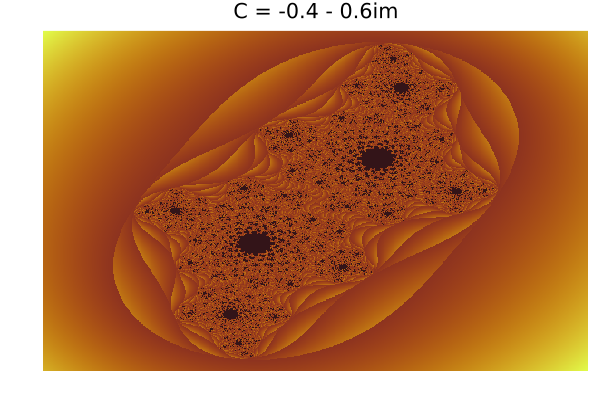
\includegraphics[scale = 0.175]{/Q1/JuliaSet1}
        \label{fig:1.1}
        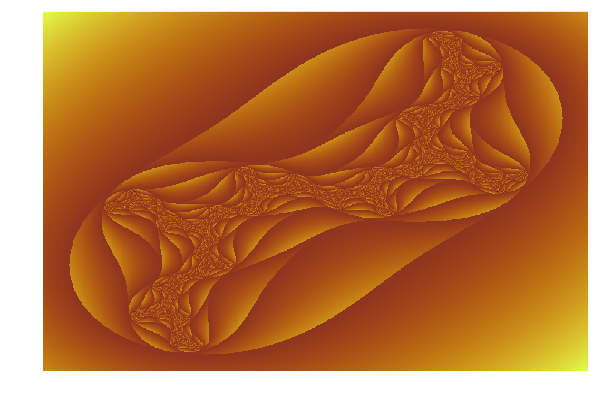
\includegraphics[scale = 0.175]{/Q1/JuliaSet2}
        \label{fig:1.2}
        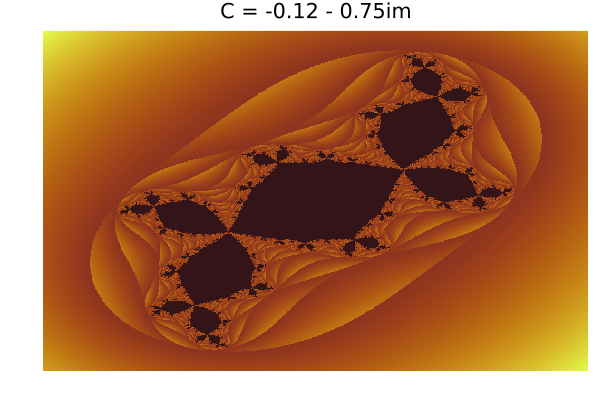
\includegraphics[scale = 0.175]{/Q1/JuliaSet3}
        \label{fig:1.3}
        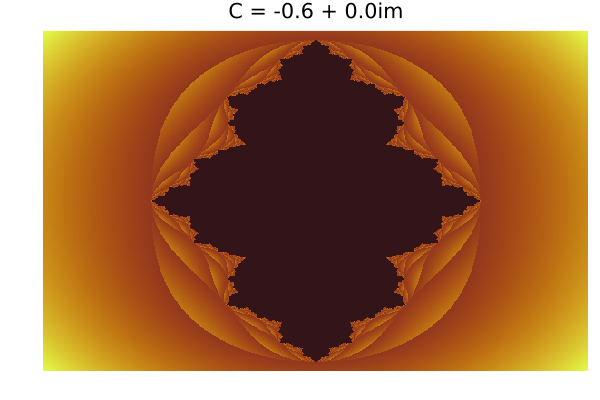
\includegraphics[scale = 0.175]{/Q1/JuliaSet4}
        \label{fig:1.4}
        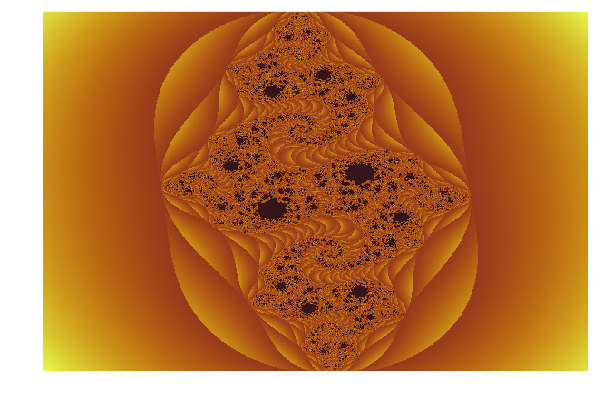
\includegraphics[scale = 0.175]{/Q1/JuliaSet5}
        \label{fig:1.5}
        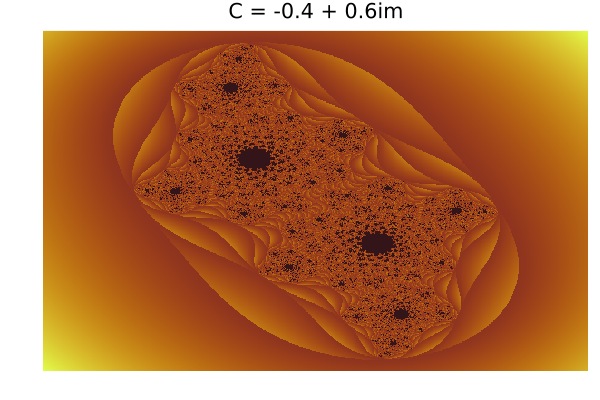
\includegraphics[scale = 0.175]{/Q1/JuliaSet6}
        \label{fig:1.6}
        \caption{Julia set fractals. you're seeing the result of the simulation of Julia set for
        the mentioned values of C.}
    \end{figure}

    \pagebreak
    
    \section*{Problem 2}
    \textbf{Basic description:}

    Now we want to simulate the Random ballistic deposition.
    We have a surface that we discredited in some equal portions
    and some time step that in each step,
    a certain number of particles will be deposed.
    If the time intervals are equal then we introduce
    the number of particles as "Rate". So if we define $S_{f}$
    as total time steps, then the number of total particles
    that deposed will be equal to $S_{f}\times Rate$. The results are shown in three plots.
    the first one is the graphical view of the whole deposition over time.
    the second one is the $\overline{H}_{(t)}$ plot over time. and the third one is
    the log-log plot of $W_{(t)}$ over time.

    The rates of each simulation are different.
    The first plot simulation rate is equal to 10000 particles per time.
    The second plot has a rate of 5000 over 20 time-steps and the last plot has a rate of 10.
    The length of surface for all of three plots is equal to 200.


    We must note that the last plot is a log-log plot so the time intervals
    are different from each other and will be grown logarithmic.
    Also, plots have error bars but accuracy made them small.
    The size of error bars is calculated after 1000 times run.

    The results:

    \begin{figure}[!htb]
        \centering
        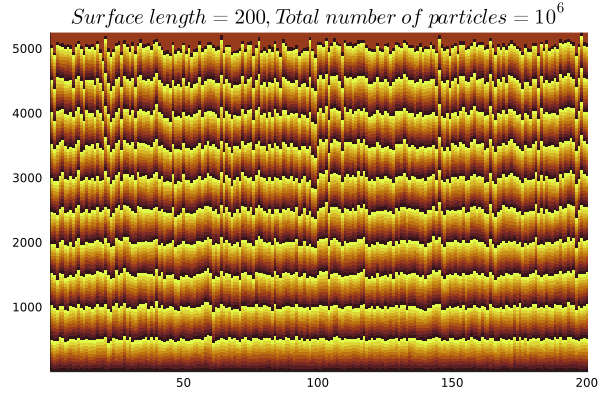
\includegraphics[scale = 0.4]{/Q2/RBDGr}
        \label{fig:2.1}
        \caption{The graphical view of deposition.}
    \end{figure}
    \pagebreak
    \begin{figure}[!htb]
        \centering
        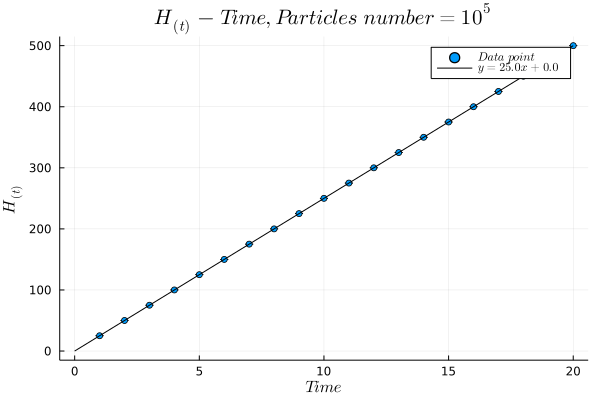
\includegraphics[scale = 0.28]{/Q2/RBDH(t)}
        \label{fig:2.2}
        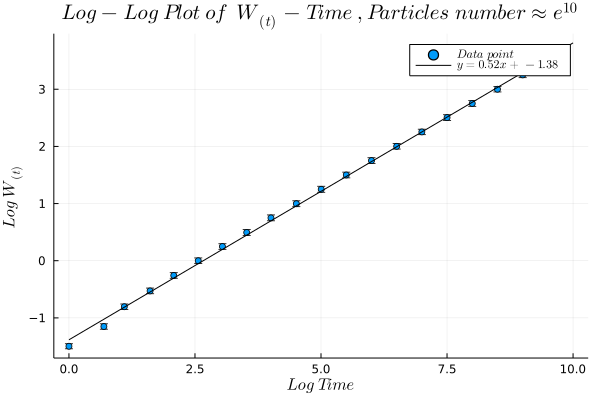
\includegraphics[scale = 0.28]{/Q2/RBDW(t)}
        \label{fig:2.3}
        \caption{The amount of the $W_{(t)}$ and $\overline{H}_{(t)}$ over time.}
    \end{figure}

    As you can see, the line slope in the log-log is equal to 0.52. So the $\beta$ is equal to 0.52.
    The line slope of $\overline{H}_{(t)}$ is equal to $rate \div surface length$ = 25.

\end{document}